\chapter{Testy sposobów komunikacji radiowej}
\label{cha:teoria}

Testy mają na celu zbadać skuteczność wyznaczania odległości między transmiterem, a odbiornikiem dla sygnałów Wifi i Bluetooth.\\
Testy odbywać się będą w dwóch etapach:
\begin{itemize}
	\item w pierwszym, odbiornik i transmiter będą oddalone od siebie o około 1m. Mierzona będzie siła odbieranego sygnału. Celem tego etapu jest określenie, jak duże straty siły sygnału wziązane są z komunikacją Wifi i Bluetooth. Straty mogą wynikać z izolacji obudowy, odbić, interferencji kilku fal lub z braku kierunkowości anteny (antena wbudowana).
	\item w drugim etapie, obliczone wcześniej wartości strat zostaną wykorzystane aby zmierzyć, jak zmienia się siła sygnału, kiedy na drodze pojawi się przeszkoda. Do testów wykorzystana została książka o formacie A4, której grubość nie przekracza kilka centymetrów
\end{itemize}
Uzyskane informacje pozwolą obliczyć współczynnik strat, jaki należy uwzględnić podczas późniejszego obliczania lokalizacji użytkowników oraz pozwoli przydzielić każdemu ze sposobów komunikacji radiowej odpowiednią wagę, w zależności od jego odporności na zakłócenia.
\section{Wykorzystane urządzenia}
\begin{enumerate}
	\item Smartphone Sony Xperia Z1 Compact (D5503) - odbiornik\\				
	Dane techniczne:
	\begin{itemize}
		\item Częstotliwość - 2,4GHz
		\item Przyrost siły sygnału z anteny WiFi - 2dBi
		\item Przyrost siły sygnału z anteny Bluetooth - 0dBi
	\end{itemize}
	\item Router TP-Link TD-W8970 - nadajnik\\
	Dane techniczne:
	\begin{itemize}
		\item Częstotliwość - 2,4GHz
		\item Dwie zewnętrzne anteny kierunkowe
		\item Przyrost siły sygnału z anteny - 4dBi
		\item Siła transmitera - 16.5dBm					
	\end{itemize}
	%\item Router TP-Link TL-WA701ND - nadajnik\\
	%Dane techniczne:
	%\begin{itemize}
	%	\item Częstotliwość - 2,4GHz
	%	\item Jedna zewnętrzna antena kierunkowa
	%	\item Przyrost siły sygnału z anteny - 2dBi
	%	\item Siła transmitera - 15dBm					
%	\end{itemize}
	\item Smartphone Samsung Grand 2 (G7102) - nadajnik\\
	Dane techniczne:
	\begin{itemize}
		\item Częstotliwość - 2,4GHz
		\item Jedna antena wbudowana
		\item Przyrost siły sygnału z anteny - 0dBi
		\item Siła transmitera Wifi - 10dBm
		\item Siła transmitera Bluetooth - 2dBm				
	\end{itemize}
\end{enumerate}
\section{Warunki}
Wszystkie pomiary wykonywane były w pomieszczeniu zamknięty, bez przeszkód na drodze sygnału. Wszystkie urządzenia znajdowały się na tej samem wysokości, skierowane do siebie górną częścią (w przypadku routeru, skierowany był on do odbiornika swoimi antenami kierunkowymi).
\section{Wyznaczenie wartości strat}
Eksperyment polegał na ustawieniu transmitera 1m od odbiornika na jednym poziomie, antenami do siebie. Na podstawie siły sygnałów obliczana była wartość strat, jakie musiałyby być uwzględnione, aby odległość obliczona równała się odległości fizycznej.\\			
\begin{figure}[H]
	\centering			
	\caption{Szkic eksperymentu nr 1}
	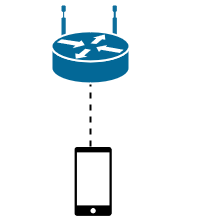
\includegraphics{exper1}
\end{figure}
\subsection{Wifi}
	Wartości obliczone dla eksperymentu nr 1, w którym Router TP-Link TD-W8970 jest transmiterem sygnału Wifi:
	\begin{center}
		\begin{minipage}{\linewidth}
			\begin{tabular}{|c|c|c|}
				\hline 
				Pomiar & Siła sygnału (w dBm) & Obliczona wartość strat (dB) \\ 
				\hline 
				1 & -41 & 24 \\ 
				\hline 
				2 & -40 & 23 \\ 
				\hline 
				3 & -37 & 20 \\ 
				\hline 
				4 & -42 & 25 \\ 
				\hline 
				5 & -37 & 20 \\ 
				\hline 
			\end{tabular} 
		\end{minipage} 
	\end{center}
Średnia arytmetyczna wartości strat dla komunikacji przy użyciu WiFi wynosi 22,4 dB.
\subsection{Bluetooth}
Wartości obliczone dla eksperymentu nr 1, w którym smartphone Samsung Grand 2 jest transmiterem sygnału Bluetooth:
\begin{center}
	\begin{minipage}{\linewidth}
		\begin{tabular}{|c|c|c|}
			\hline 
			Pomiar & Siła sygnału (w dBm) & Obliczona wartość strat (dB) \\ 
			\hline 
			1 & -59 & 31 \\ 
			\hline 
			2 & -61 & 33 \\ 
			\hline 
			3 & -57 & 29 \\ 
			\hline 
			4 & -58 & 30 \\ 
			\hline 
			5 & -58 & 30 \\ 
			\hline 
		\end{tabular} 
	\end{minipage} 
\end{center}
Średnia arytmetyczna wartości strat dla komunikacji przy użyciu Bluetooth wynosi 30,6 dB.
\subsection{Wnioski}
Opierając się na wynikach uzyskanych podczas eksperymentów wynika, że straty wynikające z zakłóceń sygnału Bluetooth są wyższe niż wynikające z zakłóceń sygnału WiFi. Może się to wziązać z tym, że transmiter Wifi ma większą moc, zaś kierunkowe anteny zmniejszają ilość zakłóceń wynikających z oblicia się sygnału. Wartości strat obliczone dla obu sposobów komunikacji zostaną wykorzystane podczas eksperymentu nr 2.